\chapter{Introducción}
\chapterquote{Avanza rápido el tema de las tortugas}{D. H. Zanette}
 
\section{Motivación}
El movimiento de los animales es de fundamental importancia para procesos ecológicos. Los humanos han estado interesados en el movimiento individual y poblacional por milenios. Hace más de 2000 años, Aristoteles escribió acerca del movimiento de los animales y los conceptos filosóficos y matemáticos asociados, en su libro, \textit{De Motu Animalium.} Históricamente, era crucial entender su comportamiento para saber cómo y dónde se podían obtener estas fuentes de alimento salvajes. Por lo tanto, los primeros humanos eran modeladores naturales del movimiento animal.  En tiempos modernos, estamos interesados en su movimiento por razones científicas y para poder tomar medidas de conservación y protección.
 
 
 
La mayoría de las especies animales son capaces de realizar complejos patrones de movimientos que generalmente dependen del ambiente, factores intrínsecos de los individuos y las interacciones entre ellos (\cite{morales2005adaptive}, \cite{morales2010building} y \cite{nathan2008emerging}). La complejidad de estos movimientos están manifestados en sus trayectorias. %Para el caso de las tortugas estas trayectorias dependen fuertemente de la vegetación en la zona de estudio y la época del año (caso que busquen reproducirse, depositar sus huevos, etc.).
 
 
 
\section{  \textit{Chelonoidis chilensis} }
\label{C chilensis}
 
Nuestra especie de interés es la tortuga $Chelonoidis$ $chilensis$, que se distribuye desde el Gran Chaco hasta el norte de la Patagonia, como se muestra en la Fig.~\ref{fig:distribuciondeEspecie} (\cite{chebez2008se}). Esta especie está incluida en el apéndice de la \textit{Convention on International Trade in Endangered Species of Wild Fauna and Flora (CITES)} y fue categorizada como \textit{vulnerable} a nivel nacional \cite{prado2012categorizacion} e internacional por la \textit{International Union for Conservation of Nature (IUCN)}.
Los principales factores que llevaron a esta situación son la reducción, modificación y destrucción de su hábitat, debido a la expansión de la frontera agropecuaria, así como su comercialización, siendo la especie nativa de reptiles más ilegalmente traficada en el mercado de mascotas en Argentina \cite{prado2012categorizacion}. Además, la amenaza a esta especie se ve aumentada con la introducción de especies depredadoras exóticas como el Jabalí (\textit{Sus scrofa}) \cite{kubisch2014chelonoidis}. En este trabajo estudiaremos una población de tortugas en en el límite sur de su distribución geográfica, a 20 km al norte de San Antonio Oeste, provincia de Río Negro, Argentina.  \\
   
Las tortugas son animales  herbívoros que se alimentan con tallos y frutos de cactus (\textit{Opuntia sulphurea, Cereus aethiops, Perocactus tuberosus}), gramíneas (\textit{Chloris castilloniana, Trhichloris crinita}), herbáceas (\textit{Alternanthera pugens, Sphaeralcea miniata, S. mendocina, Portulaca grandiflora}) y vainas de leguminosas \cite{zacarias2016biologia}.
   
   
   
\begin{figure}[ht]
    \begin{center}
        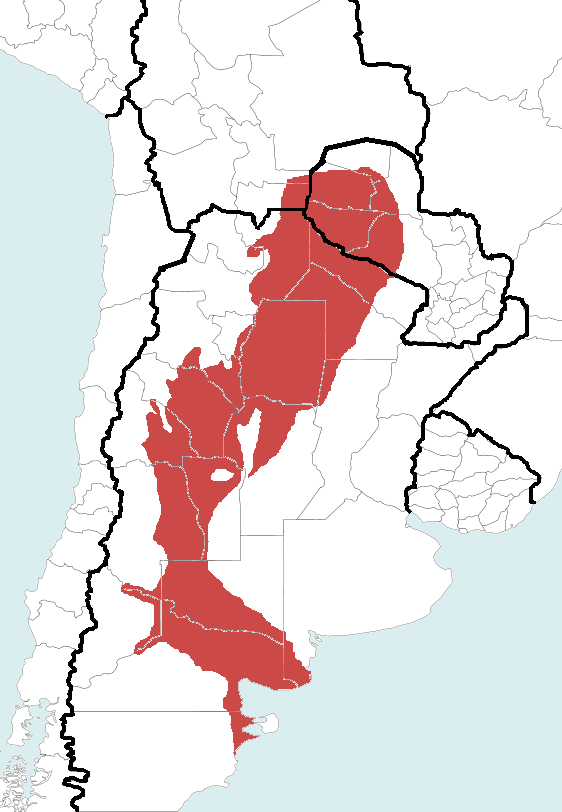
\includegraphics[width=\imsize]{figs/Chap1/Chelonoidis_chilensis_geographic_range.png}
        \caption[Distribución geográfica de la especie de tortuga \textit{Chelonoidis chilensis}.]{Distribución geográfica de la especie de tortuga \textit{Chelonoidis chilensis}
        . En este trabajo estudiaremos una población de tortugas en en el límite sur de su distribución geográfica, a 20 km al norte de San Antonio Oeste, provincia de Río Negro, Argentina.}
        \label{fig:distribuciondeEspecie}
        \end{center}
\end{figure}
Esta especie presenta un dimorfismo sexual cuando son adultos, siendo los machos notablemente más chicos que las hembras. El período de actividad (en la distribución más sur) de la especie a las latitudes de la zona de estudio es el más corto, ya que durante el invierno  bruman (parecido a hibernar) por aproximadamente cinco meses. Sus períodos de actividad comienzan durante la primavera, en el mes de septiembre. Desde noviembre a diciembre, ocurren los apareamientos; y entre enero y marzo es cuando las hembras pasan una gran parte del tiempo buscando un lugar adecuado para enterrar sus huevos \cite{Erika}. Al momento se conoce muy poco sobre la dinámica poblacional de C. \textit{chilensis} presente en Argentina.
 
Motivados por la falta de información, el objetivo de este estudio es caracterizar el movimiento y las interacciones de las tortugas en una de las poblaciones en el límite sur de su distribución geográfica. Aprender acerca del movimiento de los individuos es fundamental para entender su rol ecológico en el ecosistema y para diseñar políticas de conservación de la especie y su hábitat.
 
 
\section{Metodologías}
 
Se combinaron diferentes técnicas para monitorear las trayectorias de las tortugas. Para este trabajo se utilizaron datos recolectados por  el grupo de investigación (Física Estadística e Interdisciplinaria) en cuatro campañas de medición realizadas entre enero de 2020 y mayo del 2022.
 
En primer lugar se utilizó la técnica de radiotelemetría para la localización de la posición de las tortugas. En segundo lugar, se utilizó una unidad de navegación (construída en el Centro Atómico Bariloche), para registrar señales de GPS y contaba con sensores inerciales y de temperatura. En tercer lugar, más recientemente en el año 2022 se comenzó a utilizar un datalogger comercial (i-gotU GT120) que toma datos de GPS y hora. En las siguientes subsecciones se proveerán más detalles de ambas metodologías.
 
\subsection{Radiotelemetría}
La técnica de radiotelemetría permite localizar individuos mediante un sistema de transmisor-receptor-antena. Se utilizaron transmisores Holohil (Grand HOLOHIL Systems Ltd. RI-2B) pegados a los caparazones de las tortugas mediante cinta adhesiva. Estos transmisores emiten un pulso a una determinada frecuencia ($\approx$150 MHz) cada dos segundos. Los pulsos eran detectados por un sistema de recepción, que consiste en una antena Yagi-Uda conectada a un receptor ATS R410 (Advanced Telemetry Systems,Inc). Esta técnica permite con gran precisión localizar el transmisor y, usando un GPS portátil (Garmin eTrex
x20), determinar la ubicación de la tortuga.
 
A pesar de ser muy precisa espacialmente, esta técnica no posee una buena resolución temporal, necesaria para reconstruir trayectorias confiables. En primer lugar, es necesario seguir constantemente al individuo para tener una mejor resolución temporal. En segundo lugar, el investigador debe acercarse a una distancia considerable de la tortuga para tomar su posición con el GPS. Ambos factores pueden alterar el comportamiento de la tortuga y su trayectoria. En la siguiente sección se describe la unidad de navegación, que ofrece una alta resolución temporal en las trayectorias sin perturbar al comportamiento animal. Es por esta razón que solo se usó esta técnica para recuperar la unidad de navegación y el i-gotU, no para monitorear la trayectoría directamente.
 
\subsection{Unidad de navegación}
Se desarrolló en el departamento de Ingeniería del Centro Atómico  una unidad de bajo presupuesto para monitorear individuos en su hábitat natural (de ahora en más llamado tortugómetro), que consiste de un receptor GPS, sensores inerciales (acelerómetro y giróscopo) y un sensor de temperatura (Fig.~\ref{fig:tortugometro}). El mismo está alimentado por una batería recargable que le da una autonomía de aproximadamente 15 horas considerando una adquisición del GPS de un punto cada 5-10 minutos. El peso del tortugómetro es de 45 g representando el 3\% del peso de una tortuga de tamaño medio, lo que es aceptable para no disturbar el movimiento del animal. Los datos del receptor de GPS y de los sensores inerciales son guardados en una memoria micro-SD. Al final de cada día de monitoreo se descargaron los datos de la memoria y se cargaron las baterías.
 
En este trabajo, se utilizaron datos obtenidos por campañas realizadas por el grupo de investigación. Se contó con 8 de estas unidades en correcto funcionamiento para monitorear las tortugas en cada día de campaña. Las campañas de medición donde se utilizó esta técnica fueron entre enero de 2020 y enero del 2022. Se monitorearon en total 27 individuos por un total de 1160 horas.
\begin{figure}[ht]
    \begin{center}
       
   
    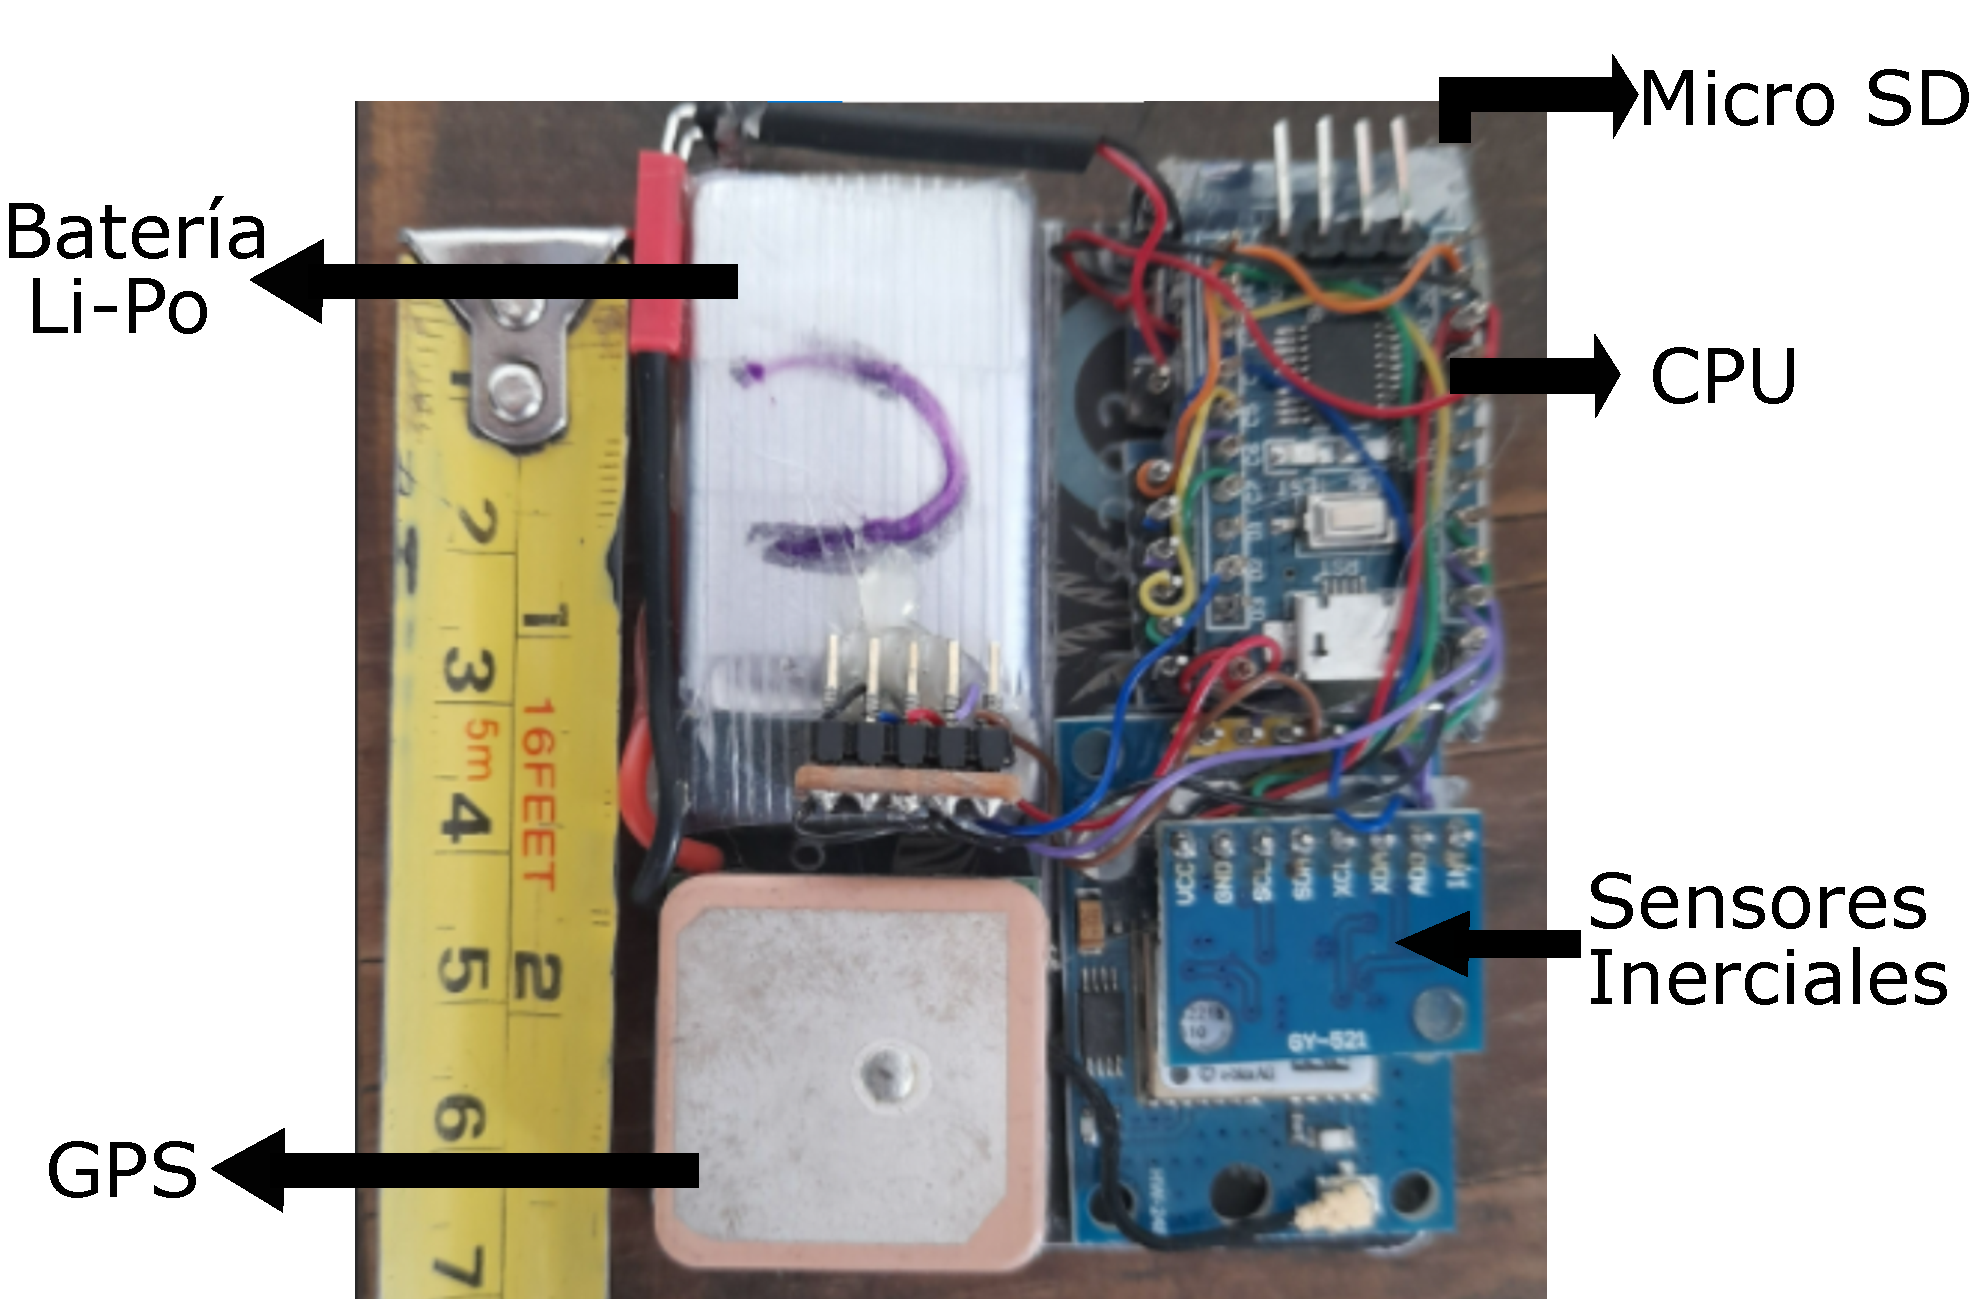
\includegraphics[width=\imsize]{figs/Chap1/tortugometro.pdf}  
\end{center}
    \caption[Unidad de navegación (tortugómetro) para monitorear individuos.] {Unidad de navegación (tortugómetro) para monitorear individuos. Consiste de un GPS, sensores inerciales (giróscopo y acelerómetro) y de temperatura, todos conectados a una unidad de control y procesamiento. Pesa menos de 45g. Las posiciones del GPS son adquiridas cada 10 minutos y se almacenan en la tarjeta micro SD extraíble. }
    \label{fig:tortugometro}
\end{figure}
 
\subsection{i-gotU}
La unidad de navegación comercial i-gotU GT120 (Fig.~\ref{fig:igotu}) es una unidad de bajo costo que permite monitorear la posición de individuos en su hábitat natural. La misma posee un receptor GPS, donde se puede programar la frecuencia de medición a través de un software provisto por el fabricante. La batería de la unidad permite una autonomía de aproximadamente 7 días. El peso de la unidad es de 21 g, lo que representa el 1.5\% del peso de una tortuga de tamaño medio. La unidad  posee una memoria interna que almacena los datos de posición y hora. Los datos se pueden descargar a la computadora a través de un puerto USB.
 
\begin{figure}[ht]
    \begin{center}
       
   
    
\includegraphics[width=.8\imsize]{figs/Chap1/igotu.jpg}  
\end{center}
    \caption[Unidad de navegación comercial i-gotU para monitorear individuos.] {Unidad de navegación i-gotU para monitorear individuos. Pesa aproximadamente  21\,g, las posiciones del GPS son adquiridas cada 15 minutos y se almacenan en la memoría interna del dispositivo. }
    \label{fig:igotu}
\end{figure}
Con este dispositivo se obtuvieron datos de campañas realizadas entre finales de enero 2022 y abril 2022, se contaron con 12 de estas unidades en correcto funcionamiento y se decidió monitorear a las mismas 6 tortugas intercambiando el i-gotU a cada una de ellas cada 7 días. Se programaron los i-gotU para adquirir posición y hora cada 15 minutos entre las 6 de la mañana y las 9 de la noche, sobre la noche no adquiere datos para ahorrar batería. En total se monitorearon aproximadamente 1000 horas por tortuga ya que algunas semanas no se llegó a intercambiar los i-gotU.
 
\section{Redes complejas}
El uso de herramientas de redes complejas permitió comparar resultados provenientes de diferentes análisis sobre los datos de GPS de las tortugas. En este trabajo se utilizaron métricas sobre la topología de distintas redes generadas, todas calculadas utilizando  funciones implementadas en la librería networkX de Python \cite{networkx}.
 
Una red compleja es un conjunto de elementos (nodos) conectados entre sí por enlaces (aristas). La topología de una red compleja puede ser estudiada a través de distintas métricas. En este trabajo se utilizaron las siguientes métricas:
\begin{itemize}
    \item \textbf{Densidad}: es la fracción de enlaces que existen en la red respecto de la cantidad de enlaces que podrían existir en la red. Se calcula como:
    \begin{equation}
        \rho = \frac{2m}{n(n-1)},
    \end{equation}
    donde $n$ es la cantidad de nodos y $m$ la cantidad de enlaces.
    \item  \textbf{Modularidad}: es una medida de fuerza de división de la red en comunidades. Se calcula como:
    \begin{equation}
        Q = \sum_{c=1}^{n}
        \left[ \frac{L_c}{m} - \gamma\left( \frac{k_c}{2m} \right) ^2 \right]
    \end{equation}
    donde $L_c$ es la cantidad de enlaces que conectan nodos de la comunidad $c$, $k_c$ es la cantidad de enlaces que conectan nodos de la comunidad $c$ con nodos de otras comunidades, $m$ es la cantidad de enlaces en la red y $\gamma$ es un parámetro que depende de la red. En este trabajo se utilizó $\gamma = 1$. Las comunidades en la red se identificaron a través de un método de propagación de etiquetas semi-síncrono \cite{cordasco2010community}.
    \item \textbf{Coeficiente de agrupamiento}: es una medida de la densidad de enlaces entre los vecinos de un nodo. Se calcula como:
    \begin{equation}
        c_u = \frac{2 T(u)}{deg(u)(deg(u)-1)},
    \end{equation}
    donde $T(u)$ es la cantidad de triángulos formados por los vecinos de $u$ y $deg(u)$ es la cantidad de vecinos de $u$ (grado de $u$).
 
   \item \textbf{Centralidad de grado}: para un nodo $v$, la centralidad de grado es la fracción de nodos a la que está conectado. Se calcula como:
    \begin{equation}
        C_G(v) = \frac{deg(v)}{n-1},
    \end{equation}
    donde $deg(v)$ es el grado del nodo $v$ y $n$ es la cantidad de nodos en la red. Da una idea de la importancia relativa de un nodo en la red.
 
\end{itemize}
En los siguientes capítulos se analizarán los datos obtenidos, a través de las metodologías mencionadas, mediante el enfoque de redes complejas.
 
 
 
%%% Local Variables:
%%% mode: latex
%%% TeX-master: "template"
%%% End:
 
 
 
 
 
 

